\begin{itemize}
    \item{
		\textbf{Dot product:} 
			\begin{itemize}
				\item{ El producto escalar de dos vectores $\overrightarrow{v}$ y $\overrightarrow{w}$
					puede verse como una magnitud de cu\'an similares son sus direcciones. Se define como
					$$ \overrightarrow{v} \cdot \overrightarrow{w} = 
					|| \overrightarrow{v}|| || \overrightarrow{	w}|| \cos \theta $$
		
                    donde $|| \overrightarrow{v}||$ y $ || \overrightarrow{w}|| $
					son las normas de los vectores y $\theta$ es el \'angulo entre $\overrightarrow{v}$ y 
					$\overrightarrow{w}$
				}
				\item{
					Ya que $\cos(-\theta) = \cos(\theta)$ el signo del \'angulo no importa y es sim\'etrico, 
					o sea $ \overrightarrow{v} \cdot \overrightarrow{w} = \overrightarrow{w} \cdot \overrightarrow{v}$
				}
				\item{
					Tomando solo $\theta \in [0, \pi] $, si $\theta < \pi / 2$ entonces $ \overrightarrow{v} \cdot \overrightarrow{w} > 0$,
					si $\theta > \pi / 2$ es negativo, y si $\theta = \pi / 2$, $ \overrightarrow{v} \cdot \overrightarrow{w} = 0$
				}
		\end{itemize}
    }
    \item{
		\textbf{Dot product:} 
			\begin{itemize}
				\item{
					El producto escalar de dos vectores $\overrightarrow{v}$ y $\overrightarrow{w}$
					puede verse como una magnitud de cu\'an perpendiculares son. Se define como
					$$ \overrightarrow{v} \times \overrightarrow{w} = 
					|| \overrightarrow{v}|| || \overrightarrow{	w}|| \sin \theta $$
				}
				\item{
					Ya que $\sin(-\theta) = -\sin(\theta)$ el signo del \'angulo importa y este  
					cambia cuando los vectores son intercambiados: $ \overrightarrow{w} \times \overrightarrow{v}
					= - \overrightarrow{v} \times \overrightarrow{w} $
				}
				\item{
					$\overrightarrow{v} \times \overrightarrow{w}$ es positivo si $\overrightarrow{w}$ est\'a 
					a la izquierda de $\overrightarrow{v}$ y negativo si est\'a a la derecha. 
				}
				\item{
					Si tomamos solo $\theta \in (-\pi, \pi]$, entonces $\overrightarrow{v} \times \overrightarrow{w}$
					es positivo si $ 0 < \theta < \pi $, negativo si $ -\pi < \theta < 0 $ y cero si $\theta = 0$ \'o 
					$\theta = \pi$, o sea, si los vectores son colineares.  
			    }
			\end{itemize}
    }
    \item{
		\textbf{Orientaci\'on:}
		Podemos usar el producto cruz para determinar la orientaci\'on relativa de tres puntos $A$, $B$ y $C$. Para 
		esto calculamos $ \overrightarrow{AB} \times \overrightarrow{AC} $. Esta expresi\'on es positiva si $C$ est\'a 
		en el lado izquierdo de $\overrightarrow{AB}$, negativa si est\'a en el lado derecho, y es igual a cero si
		$C$ est\'a sobre la recta que contiene a $\overrightarrow{AB}$.  
		
		\begin{figure}
			\centering
				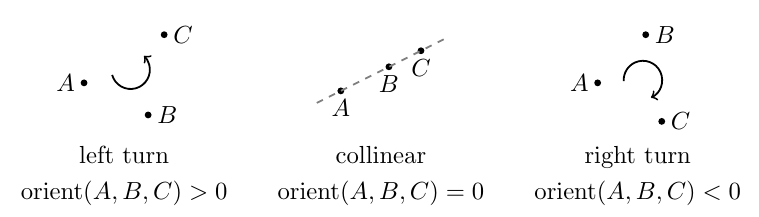
\includegraphics{imag/orient}
			\caption{Orientaci\'on Relativa}
			\label{fig:orienta}
		\end{figure}  
    }
\end{itemize}
